\documentclass[10pt,a4paper]{article}
\usepackage[utf8]{inputenc}\usepackage[T1]{fontenc}\usepackage{lmodern}
\usepackage[margin=18mm]{geometry}\usepackage{booktabs,longtable,amsmath,pgfplots}
\pgfplotsset{compat=1.18}\usepackage[hidelinks]{hyperref}\usepackage{xurl}
\setlength{\parindent}{0pt}\setlength{\parskip}{5pt}\setlength{\emergencystretch}{3em}
\title{HyMeKo: gráfalgoritmusok és generálás\\NiTech kato21 -- ellenőrzött teljesítménymérés}
\author{Core / Graph / Tensor}\date{2026-10-21 00:47 +02:00}
\begin{document}\maketitle
\textbf{Komponenskeresésben mind a hét vizsgált gráfon a HyMeKo volt gyorsabb:}
a folyamatmediánok aránya 1.88--14.94. A 35 azonos bemenetű folyamatpárból
35-ban a HyMeKo ideje volt kisebb. Ez a rögzített natív API-kra, az itt megadott
bemenetekre és gépre vonatkozó eredmény.

\textbf{330 külön folyamat, 2970 nyers minta, 66 művelet/bemenet kombináció.}
Minden kombináció öt friss folyamatban futott, folyamatonként két bemelegítéssel
és kilenc mintával. A 14 korábbi próbamérés nincs az alábbi összesítésben.
A táblázatok az öt folyamatmedián mediánját adják; a minták ismételt hívásokból
számított átlagok, nem egyedi kérések p99 késleltetései.

\section*{Azonos feladat: komponenskeresés}
Mindkét natív hívás azonos hiperél-tagságokból számol. Minden folyamatban a teljes,
közös címkézéssel normalizált partíció egyezőségét ellenőriztük. A mérés tartalmazza
a friss munkapuffert, eredménymásolást/normalizálást és az ideiglenes eredmény
felszabadítását. A gráf és a fordított incidenciaindex felépítése ezen kívül esik.
\begin{center}\begin{tabular}{lrrrr}\toprule
Eset & HyMeKo [ms] & Hypergraphz [ms] & Időarány & Nyert párok\\\midrule
A & 2.335 & 8.848 & 3.79 & 5/5 \\
B & 4.496 & 67.152 & 14.94 & 5/5 \\
C & 8.863 & 62.337 & 7.03 & 5/5 \\
D & 0.237 & 0.632 & 2.67 & 5/5 \\
E & 0.085 & 0.160 & 1.88 & 5/5 \\
F & 0.600 & 4.072 & 6.79 & 5/5 \\
G & 0.435 & 0.972 & 2.24 & 5/5 \\
\bottomrule\end{tabular}\end{center}
\begin{center}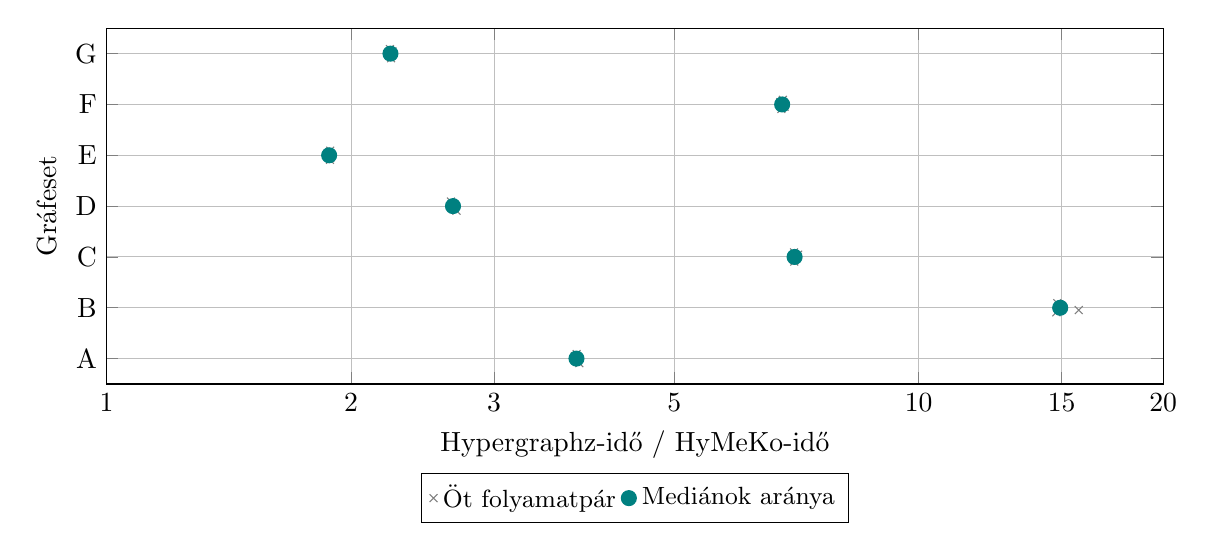
\begin{tikzpicture}\begin{axis}[
width=15cm,height=6.1cm,xmode=log,xmin=1,xmax=20,ymin=0.5,ymax=7.5,
xtick={1,2,3,5,10,15,20},xticklabels={1,2,3,5,10,15,20},
ytick={1,2,3,4,5,6,7},yticklabels={A,B,C,D,E,F,G},
xlabel={Hypergraphz-idő / HyMeKo-idő},ylabel={Gráfeset},grid=both,
legend style={at={(0.5,-0.25)},anchor=north,legend columns=2,font=\small}]
\addplot[only marks,mark=x,gray] coordinates {(3.82037556,0.9100) (3.78953898,0.9550) (3.76901126,1.0000) (3.77364124,1.0450) (3.79068938,1.0900) (14.77317912,1.9100) (15.74073810,1.9550) (14.88610992,2.0000) (14.96294222,2.0450) (14.81078637,2.0900) (7.02692324,2.9100) (7.01270084,2.9550) (7.03717692,3.0000) (7.10485531,3.0450) (7.02144400,3.0900) (2.69664670,3.9100) (2.68177380,3.9550) (2.64762453,4.0000) (2.66266185,4.0450) (2.65464158,4.0900) (1.88423773,4.9100) (1.88602625,4.9550) (1.87446547,5.0000) (1.87748119,5.0450) (1.88529301,5.0900) (6.77423943,5.9100) (6.83732460,5.9550) (6.76634694,6.0000) (6.75343172,6.0450) (6.80345440,6.0900) (2.24025811,6.9100) (2.22814123,6.9550) (2.24539633,7.0000) (2.24903016,7.0450) (2.23301620,7.0900)};\addlegendentry{Öt folyamatpár}
\addplot[only marks,mark=*,teal,mark size=2.7pt] coordinates {(3.78960833,1) (14.93598697,2) (7.03307046,3) (2.67001441,4) (1.87946324,5) (6.78981435,6) (2.23631992,7)};\addlegendentry{Mediánok aránya}
\end{axis}\end{tikzpicture}\end{center}

\newpage\section*{Pontosan milyen gráfok?}
$V$ a csúcsok, $E$ a hiperívek, $I$ az incidenciák száma. Ezekben a generált
bemenetekben egy hiperélhez egy hiperív tartozik. A C eset nyolc aktív régiót és
32768 izolált csúcsot tartalmaz. Minden eset determinisztikus; ez nem valós hálózati
adatokból származó vagy egyenletesen véletlen mintavétel.
\begin{center}\begin{tabular}{llrrr}\toprule
Jel & Család & $V$ & $E$ & $I$\\\midrule
A & Lánc & 65536 & 65535 & 131070 \\
B & Hub & 65536 & 31250 & 1000000 \\
C & 8 régió és izolált csúcsok & 65536 & 31250 & 1000000 \\
D & Steiner STS(255) & 255 & 10795 & 32385 \\
E & Teljes 3-uniform & 32 & 4960 & 14880 \\
F & Sunflower & 32769 & 1024 & 33792 \\
G & Mycielski, 7 lépés & 767 & 22196 & 44392 \\
\bottomrule\end{tabular}\end{center}
A D eset a Core Bose-konstrukciója. E minden 3-elemű részhalmaz a 32 csúcsból.
F-ben 1024 hiperél közös egyetlen csúcsban találkozik, mindegyikhez 32 saját
csúcs tartozik. G a C5 hétszeres Mycielskianja. A matematikai generátorok meglévő
Core-függvények; minden bemenet ugyanazon IrConstruction építőn megy át.

\section*{Generálás és indexelés külön}
\begin{center}\begin{tabular}{lrrr}\toprule
Eset & Generálás + IR [ms] & Index [ms] & Generálási folyamat csúcs-RSS [MiB]\\\midrule
A & 20.270 & 1.555 & 205.0 \\
B & 19.988 & 4.091 & 134.7 \\
C & 20.122 & 5.607 & 134.8 \\
D & 2.426 & 0.251 & 15.2 \\
E & 1.133 & 0.058 & 8.8 \\
F & 1.638 & 0.281 & 15.1 \\
G & 5.870 & 0.197 & 41.6 \\
\bottomrule\end{tabular}\end{center}
A generálás új kanonikus IR-t hoz létre, a kombinatorikus családoknál a Core-design
előállításával együtt. A visszaadott objektum felszabadítása nincs az időzített
szakaszban. Az indexmérés egy már létező IR-ből új fordított incidenciaindexet
épít; a megőrzött eredmény pontos bijekcióját a Core validate ellenőrzi.
Ezek meleg folyamatban végzett új objektumépítések; a fájlolvasás, nyelvi parsing,
fordítás és .hymeko profilbetöltés nincs bennük.

\begin{center}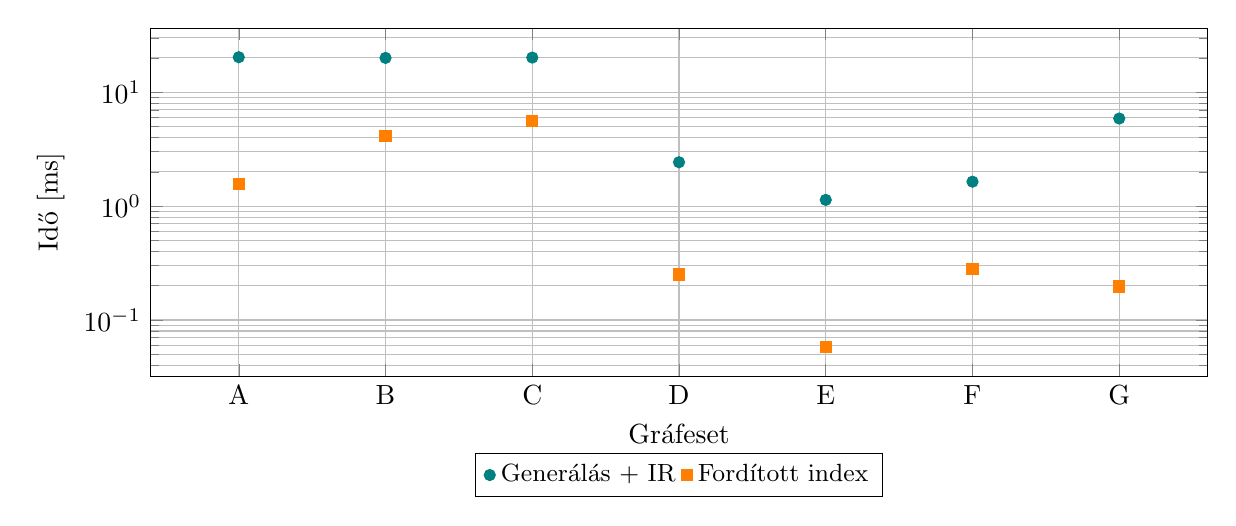
\begin{tikzpicture}\begin{axis}[
width=15cm,height=6cm,ymode=log,xtick={1,2,3,4,5,6,7},xticklabels={A,B,C,D,E,F,G},
xlabel={Gráfeset},ylabel={Idő [ms]},grid=both,
legend style={at={(0.5,-0.22)},anchor=north,legend columns=2,font=\small}]
\addplot[only marks,teal,mark=*] coordinates {(1,20.26959700) (2,19.98821500) (3,20.12197100) (4,2.42621200) (5,1.13312200) (6,1.63762600) (7,5.87001100)};\addlegendentry{Generálás + IR}
\addplot[only marks,orange,mark=square*] coordinates {(1,1.55506200) (2,4.09071900) (3,5.60675900) (4,0.25085200) (5,0.05775300) (6,0.28138300) (7,0.19658900)};\addlegendentry{Fordított index}
\end{axis}\end{tikzpicture}\end{center}

\newpage\section*{Előkészített gráfon futó algoritmusok}
Minden idő mikro\textbf{másodpercben} szerepel. A bejárás és az útkeresés a
0. csúcsból indul; az útkeresés célja a $V-1$. A duális bejárás a 0. hiperívből
indul. Az útkeresések egységköltségűek és irányítatlanok. Az A* irányított/súlyozott
változatait a helyességi szakasz ellenőrizte; ebben a teljesítménysorozatban nem mértük.
\begin{center}\begin{tabular}{lrrrrrl}\toprule
Eset & Elérhetőség & Duális & Berge/BFS & Dijkstra & Levi-bázis & Úthossz\\\midrule
A & 823.45 & 653.21 & 1783.55 & 3165.94 & 1209.21 & 65535 \\
B & 4155.84 & 3493.28 & 2845.23 & 16215.40 & 7991.78 & 1 \\
C & 476.30 & 416.81 & 486.66 & 1521.97 & 8040.12 & nincs út \\
D & 149.79 & 140.73 & 1.82 & 399.09 & 262.46 & 1 \\
E & 51.30 & 50.49 & 3.56 & 140.50 & 119.90 & 1 \\
F & 258.93 & 130.96 & 130.03 & 3371.00 & 304.81 & 1 \\
G & 213.18 & 219.62 & 5.66 & 670.26 & 387.89 & 2 \\
\bottomrule\end{tabular}\end{center}
Az útkeresésnél a teljes visszaadott út koordinátáit és lenyomatát ellenőriztük;
Dijkstra egységköltségű eredményét BFS-hosszal is összevetettük. Az elérhető halmazok
és a Levi-bázis teljes lenyomata mintánként egyezik. A munkapufferek újrahasznosulnak;
az útkeresés visszaadott útvonalának felszabadítása a mért hívás része.
A Levi-bázisra az $r=V+E-C$ rangazonosság és a függetlenség ellenőrzése is lefutott.
A C eset célja izolált: a ,,nincs út'' nem kihagyott mérés.

\section*{$s=2$ átfedés: a következő algoritmikus célpont}
Itt két hiperív akkor szomszédos, ha legalább két \emph{különböző} csúcsuk közös.
Ez más feladat, mint a fenti csúcskomponens-keresés. A jelenlegi kód minden csúcsnál
az ott találkozó ívpárokat számlálja. A mérő előre kizárja az ötmilliónál több ilyen
párt igénylő bemenetet.
\begin{center}\begin{tabular}{lrrrrr}\toprule
Eset & Idő [ms] & Komponens & Mostani párok & Csúcspár-jelöltek & Csúcs-RSS [MiB]\\\midrule
D & 130.662 & 10795 & 2040255 & 32385 & 111.8 \\
E & 227.978 & 1 & 3452160 & 14880 & 109.5 \\
F & 20.797 & 1024 & 523776 & 540672 & 34.1 \\
\bottomrule\end{tabular}\end{center}
A csúcspár-jelöltek oszlopa $\sum_e\binom{|e|}{2}$, a mostani párszám
$\sum_v\binom{d(v)}{2}$. Az itt szereplő ismétlésmentes bemeneteken ezek pontos
munkamennyiség-számok. STS(255)-nél a másik irány 63-szor, a teljes 3-uniform
esetben 232-szer kevesebb jelöltet jelent. A sunflower esetben nem kedvezőbb.

\textbf{Következő megvalósítási jelölt:} $s=2$ esetén közös csúcspárok szerint
összekapcsolni az íveket, és a két bejárási irány közül a becsült munka alapján
választani. Ez pontosan ugyanazt a kapcsolódási feltételt tudja kifejezni.
\textbf{A jelöltszám aránya nem mért gyorsulás:} az alternatív végrehajtást ebben
a szakaszban nem implementáltuk és nem mértük.

\newpage\section*{Környezet, érvényesség és reprodukció}
NiTech kato21, AMD Ryzen Threadripper 7980X, Ubuntu 24.04.3, Linux
6.14.0-37-generic. Minden mért folyamat ugyanarra a 2-es logikai CPU-ra volt kötve;
az SMT-testvért (66) a foglaltsági ellenőrzés figyelte. Nice 10, idle I/O,
16 GiB folyamatkorlát, 180 másodperces folyamat- és 15 másodperces műveletkorlát.
A mért Rust-binary Rust 1.97.1-gyel készült; a felhasználó eredeti Rust 1.96.1
telepítése változatlan maradt. Hypergraphz: rögzített natív Zig-adapter,
e45b7b80e3ce302937a56760d9fe76016ef08e26 upstream állapot.

Minden friss mérési folyamat előtt sikeres foglaltsági ellenőrzés történt.
Másik fiók jelenléténél a vezérlő mentett ellenőrzési pontból, 30 másodperces
várakozással folytatta. A figyelmeztetést kiváltó fiók \texttt{host}, UID 5069,
,,Katolab Host'' volt. Egy mintavételben SSH és automatikusan induló
systemd/pipewire/wireplumber munkamenet-szolgáltatások látszottak; másik ember
számítási munkáját ez nem bizonyítja. A fiók kapcsolatának pontos célját nem
igazoltuk, és a foglaltsági szabályt mérés közben nem lazítottuk.
Az előzetes ellenőrzés nem folyamatos külsőfolyamat-monitorozás.

\textbf{Memóriaértelmezés.} A csúcs-RSS az egész mérőfolyamaté, az előállítás és
ellenőrzés ideiglenes objektumaival együtt. A natív összehasonlításban mindkét gráf
jelen van a helyességi összevetés miatt. Ezek a számok nem egyetlen könyvtár
önálló gráftárolási méretei. A legnagyobb mért folyamatcsúcs 205.0 MiB, a
leghosszabb mérési folyamat 7.66 másodperc volt.

\textbf{Forrásazonosság.} 519 forrásfájlt SHA-256 lenyomat rögzít. Külön Linuxos
fordítási könyvtárból készült a bináris. A fordítás után két Python-fájl ellenőrzési
és összesítési javítása került be; minden Rust-forrás változatlanságát külön
ellenőriztük, majd a végleges mérési forrásállapotot ismét rögzítettük.
A Linuxos Rust-, natív egyezőségi és 31 Python-ellenőrzés sikeres volt a mérések előtt.
A lokális Clippy, Ruff, Mypy, formázás és szimbólumkapu sikeres.
Duplikáció: 543 blokk / 9100 sor, változatlan 547 / 12629 alapérték mellett.

\textbf{Mérőbináris SHA-256:} \path{0fec5d07e4253920cbe8f6132562bcd3c0bde1f6388bbb755d97e0d8f109ab8d}

\textbf{Natív könyvtár SHA-256:} \path{aa3fb04a713eeaaa8cb355ab152d12fca8a42e6a1ab0aee8a77cd59cdd7e52ea}

\textbf{Mérési forráskészlet tartalomlenyomata:} \path{4ddc05f162116d5a7e78c2f323674d7c656249821b81a3f50ecc866da1adec30}

A summary.json, measurements.csv és raw-samples.csv tartalmazza az összesítést és
mind a 2970 mintát. A download/evidence könyvtárban az eredeti folyamatnaplók,
ellenőrzési pontok, gépállapot és a 14 külön próbamérés is megmaradt.
A source-bundle.tar.gz és a korábbi build-source-bundle.tar.gz rögzíti a forrásokat;
a driver-update.json dokumentálja a fordítás utáni Python-változást.
A task-source.patch és local-validation.json az öt módosított mérő-/tesztfájl
változását és ellenőrzését írja le. Termelési gráfalgoritmus ebben a mérési
szakaszban nem változott. Függőség, commit és push nem került hozzá.
A saját távoli mérési szolgáltatások leálltak.
\end{document}
